\documentclass[tikz,border=3mm]{standalone}
\usetikzlibrary{arrows.meta,calc}

\begin{document}
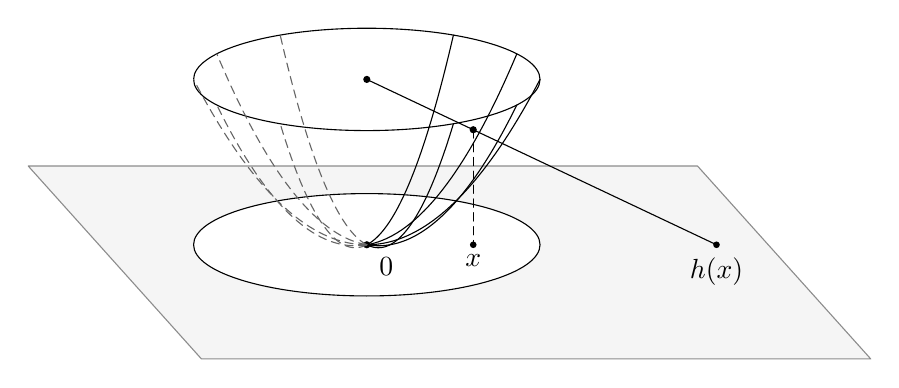
\begin{tikzpicture}[>=Stealth, line cap=round, line join=round]

% ----------------------------
% PARAMETERS
% ----------------------------
\def\a{2.2}
\def\b{0.65}
\def\H{2.1}
\def\Oy{-2.0}

\coordinate (O) at (0,\Oy);
\coordinate (Ctop) at (0,{\Oy+\H});

% ----------------------------
% BASE PLANE
% ----------------------------
\path[fill=gray!8, draw=black!45]
  (-4.3,-1.0) -- (4.2,-1.0) -- (6.4,-3.45) -- (-2.1,-3.45) -- cycle;

% ----------------------------
% PROJECTION ELLIPSE
% ----------------------------
\fill[white] (O) ellipse [x radius=\a, y radius=\b];
\draw (O) ellipse [x radius=\a, y radius=\b];

% Center
\fill (O) circle (1.3pt);
\node[below right=1pt] at (O) {$0$};

% ----------------------------
% PARABOLOID: WIRE-FRAME MERIDIANS
% z = H * r^2  with r in [0,1]
% ----------------------------

% Draw rim
\draw (Ctop) ellipse [x radius=\a, y radius=\b];

% Radial meridians (front solid, back dashed)
\foreach \ang in {-60,-30,0,30,60} {
  \draw
    plot[domain=0:1,samples=40]
    ({\a*\x*cos(\ang)},
     {\Oy + \H*\x*\x + \b*\x*sin(\ang)});
}

\foreach \ang in {120,150,180,210,240} {
  \draw[densely dashed,black!60]
    plot[domain=0:1,samples=40]
    ({\a*\x*cos(\ang)},
     {\Oy + \H*\x*\x + \b*\x*sin(\ang)});
}

% Top point
\fill (Ctop) circle (1.3pt);

% ----------------------------
% POINT ON PARABOLOID
% ----------------------------
\pgfmathsetmacro{\rP}{0.75}
\pgfmathsetmacro{\theta}{35}

\pgfmathsetmacro{\xP}{\a*\rP*cos(\theta)}
\pgfmathsetmacro{\yP}{\Oy + \H*\rP*\rP + \b*\rP*sin(\theta)}

\coordinate (P) at (\xP,\yP);
\fill (P) circle (1.3pt);

% ----------------------------
% PROJECTION x
% ----------------------------
\coordinate (x) at (\xP,\Oy);
\fill (x) circle (1.2pt);
\node[below] at (x) {$x$};

\draw[densely dashed] (P) -- (x);

% ----------------------------
% LINE THROUGH TOP AND P -> h(x)
% ----------------------------
\pgfmathsetmacro{\yC}{\Oy+\H}
\pgfmathsetmacro{\s}{(\Oy-\yC)/(\yP-\yC)}
\coordinate (hx) at ({\s*\xP},\Oy);

\fill (hx) circle (1.2pt);
\node[below=1pt] at (hx) {$h(x)$};

\draw (Ctop) -- (P) -- (hx);

\end{tikzpicture}
\end{document}
